% !TEX root=../august-boeckh-hauptdokument.tex

\chapter{Abbildungen und die Feinheiten}
\section{Drehen von Abbildungen}

% ---
% Kannst du mir den Löwen um 34° drehen?
% –
\begin{figure}[h]
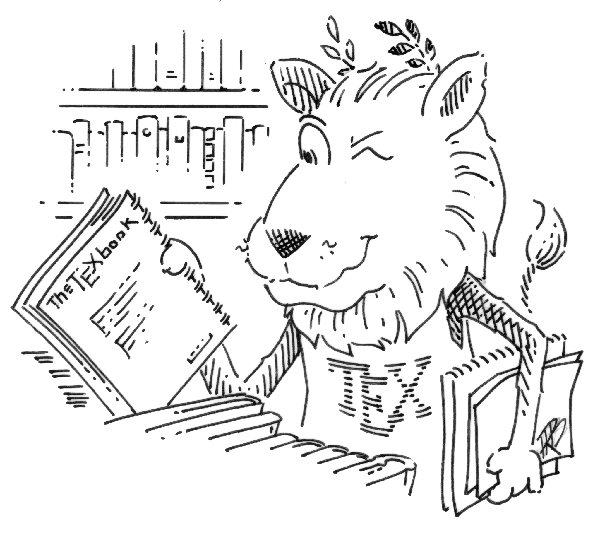
\includegraphics[trim=0cm 4cm 6cm 0cm, clip=true, width=7cm, angle=34]{figures/loewe.png}
\caption{Der \LaTeX-Löwe}
\label{fig:loewe}
\end{figure}

\ref{fig:loewe}
\mysideref{loewe}



%--
% Verweise auf Abbildungen bitte in den Seitenrand.
%--


Wilhelm von Humboldt

\begin{figure}
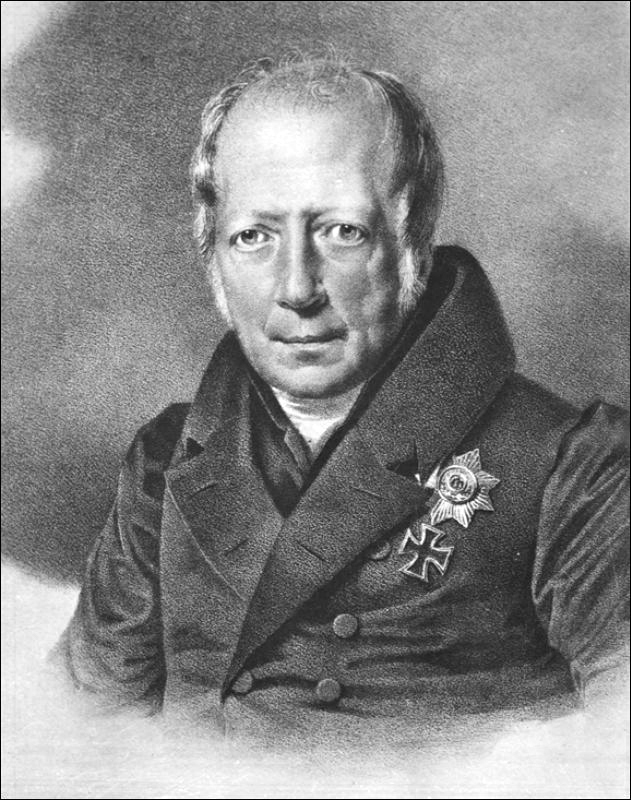
\includegraphics[width=0.4\textwidth]{wilhelm}
\caption{Wilhelmv von Humboldt (1767--1835)}
\label{fig:wilhelm}
\end{figure}
% ---
% Hier bitte das Bild von Wilhelm vH einfügen
% Datei: wilhelm
% Bildunterschrift: Wilhelm von Humbolt (1767--1835)
% ---

Friedrich Wilhelm Christian Carl Ferdinand von Humboldt (* 22. Juni 1767 in Potsdam; † 8. April 1835 in Tegel) war ein preußischer Gelehrter, Schriftsteller und Staatsmann. Als Bildungsreformer initiierte er die Neuorganisation des Bildungswesens im Geiste des Neuhumanismus und betrieb die Gründung der Friedrich-Wilhelms-Universität Berlin.

Zusammen mit seinem Bruder Alexander von Humboldt zählt er zu den großen, fortwirkend einflussreichen Persönlichkeiten in der deutschen Kulturgeschichte. Während Alexander dabei vor allem der erd- und naturwissenschaftlichen Forschung neue Horizonte erschlossen hat, lagen die Schwerpunkte für Wilhelm in der Beschäftigung mit kulturwissenschaftlichen Zusammenhängen wie der Bildungsproblematik, der Staatstheorie, der analytischen Betrachtung von Sprache, Literatur und Kunst sowie in aktiver politischer Mitgestaltung als Reformmotor im Schul- und Universitätswesen und als preußischer Diplomat.

%--
% VERWEIS auf wilhelm
%--
Siehe \ref{fig:wilhelm}

Inmitten aller Vielfalt der von aufklärerischen Impulsen bestimmten, gemeinwohlorientierten Betätigungen in Politik, Bildungswesen, Kultur und Wissenschaft hatte Wilhelm von Humboldt stets zugleich die Auslotung und Bildung der eigenen Individualität und Persönlichkeit im Blick. In der wiederum auf menschliche Individuen allgemein anzuwendenden Zielformel geht es um „die höchste und proportionierlichste Ausbildung aller menschlichen Kräfte zu einem Ganzen“.


Alexander von Humboldt
Friedrich Wilhelm Heinrich Alexander von Humboldt (* 14. September 1769 in Berlin; † 6. Mai 1859 ebenda) war ein deutscher Naturforscher mit einem weit über Europa hinausreichenden Wirkungsfeld. In seinem über einen Zeitraum von mehr als sieben Jahrzehnten entstandenen Gesamtwerk schuf er „einen neuen Wissens- und Reflexionsstand des Wissens von der Welt“[1] und wurde zum Mitbegründer der Geographie als empirischer Wissenschaft. Er war der jüngere Bruder von Wilhelm von Humboldt.

Seine mehrjährigen Forschungsreisen führten ihn nach Lateinamerika, in die USA sowie nach Zentralasien. Wissenschaftliche Feldstudien betrieb er unter anderem in den Bereichen Physik, Chemie, Geologie, Mineralogie, Vulkanologie, Botanik, Vegetationsgeographie, Zoologie, Klimatologie, Ozeanographie und Astronomie, aber auch zu Fragen der Wirtschaftsgeographie, der Ethnologie und der Demographie. Zudem korrespondierte er bei seinem publizistischen Werk mit zahlreichen international bedeutenden Spezialisten der verschiedenen Fachrichtungen und schuf so ein wissenschaftliches Netzwerk eigener Prägung.
%--
% VERWEIS auf alexander 
%--
Siehe \ref{fig:alexander}

In Deutschland erlangte er vor allem mit den Ansichten der Natur und dem Kosmos außerordentliche Popularität. Sein bereits zu Lebzeiten hohes Ansehen spiegelt sich in Bezeichnungen wie „der zweite Kolumbus“, „wissenschaftlicher Wiederentdecker Amerikas“, „Wissenschaftsfürst“ und „der neue Aristoteles“ (Gedenkmünze der Pariser Akademie der Wissenschaften). Er wurde in zahlreiche in- und ausländische Akademien aufgenommen.

\begin{figure}
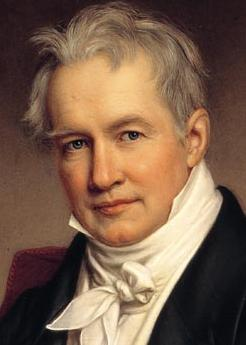
\includegraphics[width=0.4\linewidth]{alexander}
\caption{Alexander von Humboldt (1769--1859)}
\label{fig:alexander}
\end{figure}
% ---
% Hier bitte das Bild von Alexander vH einfügen
% Datei: alexander
% Bildunterschrift: Alexander von Humbolt (1769--1859)
% ---


%---
% Wie kann man die Kompiliergeschwindigkeit erhöhen?
% Kann ich die Abbildungen auch (teilweise) ausblenden?
% Kann ich auch einen „Platzhalter-Text“ anstatt des Bildes setzen?
%---




\section{Abbildungen beschriften}
%---
% Kann ich auch noch eine Beschriftung in das Bild von Wilhelm bekommen?
% Vielleicht sowas wie „LaTeX ist toll!“
% Kannst du auch noch das Bild von Alexander in das Bild von Wilhelm integrieren?
%---
\section{Ausschnitthafte Vergrößerungen bei Abbildungen}

%---
% Das Bild von Wilhelm ist ja schön und gut, 
% aber ich kann sein Abzeichen nicht richtig erkennen.
% Kannst du dieses vergrößern?
%---


